\capitulo{5}{Aspectos relevantes del desarrollo del proyecto}

En este capítulo se explican las partes más relevantes del desarrollo del proyecto, así como los problemas surgidos y las decisiones tomadas al respecto. Este apartado se ha decidido dividir en 3 secciones: el estudio previo al desarrollo del proyecto, la implementación y llenado de la base de datos, y la presentación de los datos.

\section{Estudio preliminar}
\label{sect:estudio_preliminar}

En esta fase inicial se decidió investigar las posibles herramientas a utilizar para el desarrollo del proyecto, así como desarrollar una serie de scripts para probar su funcionamiento y familiarizarse con sus interfaces de programación.

El primer paso que se llevó a cabo en esta fase del proyecto fue crear un entorno de trabajo sobre el cual poder implementar el resto de scripts del proyecto. Como se indicó en el apartado \ref{sect:otras_herramientas}, para esta tarea se decidió emplear la herramienta \texttt{virtualenv}, que nos permite crear un entorno aislado para Python de modo que se puedan fijar las versiones de las librerías descargadas en este caso mediante \texttt{pip3} a cierta versión, algo muy importante en esta fase de pruebas donde se va a probar múltiples herramientas.

Una vez creado el entorno de trabajo, la primera tarea que se decidió abordar fue investigar las posibles herramientas a utilizar para llevar a cabo la descarga de datos de la página web de Instagram. Tras hacer varias pruebas con múltiples scrapers web encontrados en GitHub como \texttt{instagram-crawler}, \texttt{huaying-instagram-crawler}, etc. se decidió emplear \texttt{Instalooter}, el cual dispone tanto de una interfaz de programación para Python 3 como de un cliente de línea de comandos. El resto de scrapers encontrados no parecían funcionar en el momento en que se hizo la prueba, posiblemente debido a que la web de Instagram hubiese sido actualizada de forma reciente y éstos programas no hubiesen sido actualizados de acorde a los nuevos cambios.

Como se comentó en la sección \ref{sect:instalooter}, Instalooter pone a disposición del usuario de varios \textit{looters}, \texttt{ProfileLooter} y \texttt{HashtagLooter}, para descargar las publicaciones relacionadas con un perfil de usuario o con un Hashtag respectivamente, y permite descargar tanto las vídeos, como imágenes como la descripción y meta-datos de las mismas en formato JSON. Una de las ventajas que tiene esta herramienta en comparación con otras es que permite comprobar si una publicación ha sido ya descargada o no para evitar repetirla, así su puede ejecutar la descarga de forma sucesiva sin riesgo de acabar con datos duplicados.

Durante las pruebas con Instalooter se pudo descargar con éxito tanto las imágenes como los meta-datos de varias publicaciones de Instagram. El JSON generado por cada publicación mediante esta herramienta cuenta con la siguiente información:

\begin{table}[H]
    \hspace*{-1.5cm}
    \centering
    \begin{tabular}{|p{0.2\textwidth}|p{0.4\textwidth}|p{0.4\textwidth}|}
    \hline
    Nombre del Campo & Ejemplo & Descripción \\ \hline
    \_\_typename & \texttt{``GraphImage''} & indica el tipo de publicación que se ha descargado, exactamente si es un vídeo o una imagen \\ \hline
    comments \_disabled & \texttt{false} & Si los comentarios de la publicación se encuentran habilitados o no \\ \hline
    dimensions & \texttt{\{``height'': 640,``width'': 640\}} & Anchura y altura de la imagen \\ \hline
    display\_url & \texttt{``https://scontent-ams2-1.
    cdninstagram.com/v/ t51.2885-15/...''} & URL de descarga de la imagen en Instagram, este link expira a los pocos días \\ \hline
    edge\_liked\_by & \texttt{\{``count'': 73\}} & Número de ``likes'' de la publicación \\ \hline
    edge\_media\_to \_caption & \texttt{\{``edges'': {[}\{``node'': \{ ``text'': ``El peso de una nube de color gris'' \}\}{]}\}} & comentario o descripción de la publicación generada por su autor \\ \hline
    \end{tabular}
\end{table}
\begin{table}[H]
    \centering
    \begin{tabular}{|p{0.2\textwidth}|p{0.4\textwidth}|p{0.4\textwidth}|}
    \hline
    edge\_media\_to \_comment & \texttt{\{``count'': 1\}} & numero de comentarios de la publicación \\ \hline
    id & \texttt{``1001662920005405392''} & número identificador de la publicación \\ \hline
    is\_video & \texttt{false} & si la publicación contiene un video o no \\ \hline
    owner & \texttt{\{``id'': ``216171681''\}} & identificador de la cuenta de instagram que hizo la publicación \\ \hline
    shortcode & \texttt{``3mnx5jmkrQ''} & Shortcode de la publicación, se puede usar para obtener un link a la publicación de forma \\ \hline
    taken\_at \_timestamp & \texttt{1433627546} & timestamp de la publicación \\ \hline
    thumbnail\_src & \texttt{``https://scontent-ams2-1.
    cdninstagram.com/v/ t51.2885-15/...'' }& URL del ``thumbnail'' de la imagen, este link expira a los pocos días \\ \hline
    \end{tabular}
    \caption{Contenido del JSON de Instalooter}
    \label{tab:json_instalooter}
\end{table}

Después de comprobar que se puede descargar con éxito publicaciones de instagram, se procedió a comprobar si es posible extraer información de las imágenes descargadas. Para ello se trató desde un principio de recurrir a herramientas ya existentes de reconocimiento de imágenes, preferiblemente de servicios en la nube.

Inicialmente por recomendación del tutor se trató de emplear los servicios de Google Cloud. Esta plataforma de Google Cloud provee diversos servicios junto con sus respectivas interfaces de programación compatibles con múltiples lenguajes de programación. Entre los servicios relevantes para el presente proyecto cabe destacar el almacenamiento en la nube con Cloud Storage, servicios de procesamiento de datos y creación de máquinas virtuales con Compute Engine, servicios de visión artificial mediante Cloud Vision, almacenamiento de bases de datos en Cloud SQL, etc.

Todos los servicios de Google Cloud se pueden probar de forma gratuita con tan solo crearse una cuenta en la plataforma. Esto es debido a que Google ofrece un crédito de 300 USD para invertir libremente en su plataforma a toda cuenta recién creada durante un periodo de 3 meses, 400 USD si se demuestra ser alumno \cite{google_cloud}. Este crédito inicial se va gastando según se vaya haciendo uso de los servicios, y una vez consumido o pasado el periodo de 3 meses, Google empieza a cobrar por el uso de sus servicios. Debido al alcance de este proyecto y los precios que tienen los servicios de Google, el anterior límite de dinero no es preocupante, aunque el de tiempo si que podría llegar a ser lo.

Como se ha comentado, para emplear los servicios de Google Cloud, Google pone a disposición de los usuarios APIs de forma gratuita para distintos lenguajes de programación, entre los cuales se encuentra Python. Mediante este lenguaje de scripting y la API de Cloud Vision \cite{api_google_vision}, se llevaron a cabo unas pruebas iniciales donde se pudo comprobar que la información que se puede obtener mediante el uso de la API de Google Cloud Vision si que incluye cierta capacidad de análisis de emociones, permitiendo obtener etiquetas de emociones como alegría, tristeza, enfado, sorpresa, etc. junto con su \textit{likelihood}, pero no incluye información como edad y género de las personas, capacidad que fue eliminada de este servicio de forma bastante reciente \cite{archive_google_gender}. Esto es un problema ya que se pretendía hacer uso de este tipo de información a la hora de recomendar publicaciones o lugares al usuario.

Debido a las anteriores limitaciones de Cloud Vision, y el problema del límite de tiempo del periodo de prueba, se decidió explorar otras alternativas. A continuación se hace un pequeño resumen de los servicios ofrecidos por las distintas alternativas valoradas y que posiblemente se puedan llegar a necesitar en el proyecto.

\begin{landscape}
\begin{table}[]
    \centering
    \resizebox{1.02\columnwidth}{0.55\textwidth}{%
        \begin{tabular}{|p{0.12\textwidth}|p{0.2\textwidth}|p{0.15\textwidth}|p{0.15\textwidth}|p{0.15\textwidth}|p{0.21\textwidth}|p{0.21\textwidth}|p{0.21\textwidth}|p{0.21\textwidth}|}
        \hline
        \multirow{2}{=}{Servicios} & \multirow{2}{=}{Límite de uso}	& \multicolumn{3}{|c|}{API de Visión Artificial}	& \multirow{2}{=}{Almacenamiento en bucket/blobs gratuito}	& \multirow{2}{=}{Almacenamiento en Base de Datos SQL}	& \multirow{2}{=}{Almacenamiento en Base de Datos NoSQL}	& \multirow{2}{=}{Máquinas Virtuales}	\\ \cline{3-5}
        	&	& Límite de uso	& Análisis de Sentimiento	& Reconoci\-miento de edad y género &	&	&	&	\\ \hline
        Google Cloud	& 300 USD durante 3 meses	& 1000 unidades al mes	& Si, con tags alegría, tristeza, enojo, sorpresa	& No	& Si, con 5 Gbs al mes en Google Cloud Storage	& Si, con motor de base de datos MySQL, PostgreSQL y SQL Server	& Si, bases de datos documentales como Cloud Datastore, Cloud Firestore... y clave/valor con MongoDB, Bigtable...	& Si, Máquina virtual en Compute Engine empleando el saldo inicial	\\ \hline
        Microsoft Azure	& 12 meses para servicios gratuitos + 200 USD para servicios no gratuitos durante 1 mes & Hasta 30.000 transacciones al mes & Si, con tags felicidad, tristeza, neutralidad, ira, desprecio, asco, sorpresa y temor	& Si	& Si, con 5 Gbs en Azure Blob Storage y 5 GBs en Azure File Storage 5 & Si, con Azure Database for MySQL (750 horas al mes), Azure Database for PostgreSQL (750 horas al mes) y SQL Database (250 Gbs)	& Si, Azure Cosmos DB (25 Gbs)	& Si, Máquina virtual B1S (1 núcleo, 1 GB RAM y 4GB de almacenamiento) con Linux 750 horas al mes	\\ \hline
        Amazon Web Services (AWS)	& 12 meses para la capa gratuita	& 5000 imágenes al mes	& Si, con tags feliz, triste, enfado, confuso, disgustado, sorprendido, calma, miedo, desconocido & Si	& Si, con 5 Gbs al mes en Amazon S3	& Si, se puede usar RDS (750 horas al mes) con motor de base de datos MySQL, MariaDB, Oracle, PostgreSQL, SQL Server y Amazon Aurora & Si, bases de datos documentales con DocumentDB (compatible con MongoDB, solo 1 mes de prueba) y clave/valor con DynamoDB (25 GB gratuitos) & Si, Máquina virtual en EC2 (1 CPU, 1GB de RAM, 1 CPU y 1GB de RAM, 30 GBs SSD) con Linux 750 horas al mes \\ \hline
        \end{tabular}%
    }
    \caption{Servicios en la Nube: Alternativas}
    \label{tab:cloud_services}
\end{table}
\end{landscape}

Cabe destacar que se seleccionaron estas alternativas en base a su popularidad, los servicios potencialmente necesarios, las restricciones de tiempo para probarlos y al requerimiento de que la plataforma usada fuera gratuita u ofreciese un periodo de prueba, ya sea para estudiantes o no, lo suficientemente extenso como para poder desarrollar el proyecto sin complicaciones. También hay que destacar que se intentó llevar a cabo pruebas con las distintas plataformas. Durante estas pruebas preliminares, con Microsoft Azure no se consiguió llegar a crear una máquina virtual de tipo \texttt{B1S} gratuita, puesto que siempre salían como no disponibles. Tras revisar la página de preguntas y respuestas de Microsoft parece que a mucha gente le ha sucedido lo mismo recientemente, el problema parece ser la alta demanda de este tipo de máquinas. Debido a este problema y la imposibilidad de obtener la edad y el género en los servicios de Google Vision, finalmente se decidió que lo mejor era emplear los servicios de \textbf{Amazon Web Services}.

Un vez tomada la decisión de la plataforma a utilizar, se procedió a hacer más pruebas con AWS. Para interactuar con cualquier servicio de Amazon Web Services, sobre todo si se hace a través de su SDK, es necesario obtener un identificador y su clave de acceso. Por lo tanto, una vez creada la cuenta lo primero que se hizo fue generar estas credenciales a través del servicio IAM (Identification and Access Management), en su apartado \textit{Credenciales de Seguridad}. Una vez generado, nos devolverá un CSV con dos valores, \texttt{AWSAccessKeyId} y \texttt{AWSSecretKey}, los cuales deberemos conservar para acceder posteriormente a los servicios.

Después de generar las credenciales se procedió a probar el servicio de Amazon Rekognition, cuyos detalles ya se introdujeron en el apartado \ref{sect:rekognition}. Para poder analizar una imagen con Rekognition, primero ésta debe de estar subida a un bucket o contenedor de objetos de Amazon S3, por ello se procedió a generar un bucket de prueba y a subir una serie de imágenes a través de la consola web. Por otro lado, para llevar a cabo pruebas con Rekognition hubo que instalar el SDK de AWS para Python, el cual es conocido como \texttt{Boto3}. Su uso a través de Python es muy sencillo, puesto que se puede acceder a cualquier servicio de AWS con tan solo usar la función \texttt{boto3.client} empleando como parámetros: el nombre del servicio a usar, la región donde se ejecuta en el servicio, que en el caso de este proyecto siempre se ha escogido ``eu-west-1'' (Irlanda), y el id y clave de acceso que anteriormente se obtuvieron mediante IAM. Durante las pruebas con Rekognition se pudo comprobar que mediante su funcionalidad de reconocimiento facial se puede obtener un JSON que contiene un array ``FaceDetails'' con un objeto por cara presente en la imagen. Cada uno de estos objetos cuenta con los siguientes detalles:

\begin{table}[H]
    \centering
    \begin{tabular}{|p{0.2\textwidth}|p{0.4\textwidth}|p{0.4\textwidth}|}
    \hline
    Nombre del Campo & Ejemplo & Descripción \\ \hline
    BoundingBox & \texttt{\{``Width'': 0.0358, ``Height'': 0.0476, ``Left'': 0.3780, ``Top'': 0.6708\}} & coordenadas de la caja donde se ubica la cara \\ \hline
    AgeRange & \texttt{\{``Low'': 49, ``High'': 57\}} & Rango de edad de la persona en años \\ \hline
    Smile & \texttt{\{``Value'': false, ``Confidence'': 94.6054\}} & Si la persona se encuentra sonriendo o no \\ \hline
    Eyeglasses & \texttt{\{``Value'': false, ``Confidence'': 97.4112\}} & Si la persona lleva o no gafas o no \\ \hline
    Sunglasses & \texttt{\{``Value'': false, ``Confidence'': 99.9965\}} & Si la persona lleva o no gafas de sol o no \\ \hline
    Gender & \texttt{\{``Value'': ``Female``, ``Confidence'': 68.2432\}} & Género de la persona \\ \hline
    Beard & \texttt{\{``Value'': false, ``Confidence'': 62.0366\}} & Si la persona tiene barba o no \\ \hline
    Mustache & \texttt{\{``Value'': false, ``Confidence'': 94.0625\}} & Si la persona tiene bigote o no \\ \hline
    EyesOpen & \texttt{\{``Value'': false, ``Confidence'': 99.8537\}} & Si la persona tiene los ojos abiertos o no \\ \hline
    MouthOpen & \texttt{\{``Value'': false, ``Confidence'': 93.5364\}} & Si la persona tiene la boca abierta o no \\ \hline
    Emotions & \texttt{{[} \{``Type'': ``SAD``, ``Confidence'': 99.9044\}, \{``Type'': ``CALM``, ``Confidence'': 23.9581\}... \} {]}} & Un array con la confianza de las emociones expresadas por la persona basada en su expresión facial. Los posibles valores son triste, calmado, sorprendido, aterrado, confundido, enfadado, feliz, disgustado. \\ \hline
    Landmarks & \texttt{{[}\{``Type'': ``eyeLeft``, ``X'': 0.3885, ``Y'': 0.6877\},\{``Type'': ``eyeRight``, ``X'': 0.4037, ``Y'': 0.6898\}...{]}} & Coordenadas de las características de la cara (nariz, boca, etc.). \\ \hline
    Pose & \texttt{\{``Roll'': 8.8927, ``Yaw'': 1.8882, ``Pitch'': 0.5692\}} & Pose (rotación) de la cara. \\ \hline
    Quality & \texttt{\{``Brightness'': 63.9795, ``Sharpness'': 4.3748\}} & Indican el brillo y nitided de la imagen \\ \hline
    Confidence & \texttt{99.8897} & Nivel de confianza en el que se encuentra una cara dentro de la caja. \\ \hline
    \end{tabular}
    \caption{Contenido del JSON de Rekognition para detección facial}
    \label{tab:json_rekognition}
\end{table}

Una vez elegidas las herramientas a utilizar, comprobado su funcionamiento y los datos que se pueden obtener, se puede concluir que es posible llevar a cabo la descarga de datos de Instagram y el procesamiento de las imágenes.

\section{Diseño e implementación de la base de datos}
\label{sect:dis_impl_bbdd}

En este apartado se explica la base de datos diseñada, y los scripts implementados para la descarga, procesado y almacenamiento de los datos generados mediante Instalooter y Rekognition de forma automática.

Como se ha comentado en el apartado anterior, se va a emplear Instalooter para la descarga de publicaciones de Instagram. Desde un principio se decidió emplear una lista de hashtags de los cuales descargar publicaciones relacionadas con Valladolid, ya que estas suelen estar etiquetadas con hashtags relacionados a eventos o lugares de la ciudad. De esta lista se hablará posteriormente. Por lo tanto, en nuestros scripts de descarga se va a emplear el looter \texttt{HashtagLooter} para este cometido, limitando la descarga de publicaciones solo a imágenes.

Una vez que se obtengan las publicaciones, antes de almacenar cualquier información en la base de datos se va a llevar a cabo el procesamiento de las imágenes mediante Rekognition para así tener la información completa. Pero como se comentó anteriormente, para ello primero las imágenes han de estar subidas a Amazon S3. Por lo tanto, primero se ha de conseguir subir las imágenes descargadas por Instalooter a Amazon S3 de forma automática. Esto inicialmente podría parece una tarea sencilla, solo tendríamos que descargar la imagen y meta-datos de una publicación de forma local, subirlo mediante boto3 a Amazon S3, y borrarlo del almacenamiento local. Pero como se comentó en la sección \ref{sect:instalooter}, Instalooter antes de descargar una publicación primero comprueba si ya existe en el directorio donde se pretende guardar, para así acelerar el proceso de \textit{scraping} y poder ejecutar Instalooter sobre un hashtag o perfil sucesivamente evitando tener publicaciones duplicadas. Esto es un problema ya que nos obliga a que el equipo que ejecute Instalooter tenga que mantener almacenadas todas las publicaciones ya descargadas, teniendo los datos duplicados en S3 y en el equipo, y dependiendo del volumen de publicaciones esto puede dar problemas de escalabilidad.

Tras revisar el código fuente de Instalooter se pudo comprobar se puede pasar una objeto que herede de la interfaz \texttt{fs.base.FS} de \textit{PyFilesystem} en vez de una ruta al sistema de archivos local, aunque esto no se encuentra documentado en su página web. Este objeto permite abstraerse del sistema de archivos local, y por ello, se pensó que tal vez se podría usar un objeto implementase esta interfaz junto con las comunicaciones con Amazon S3, para así no tener que usar el almacenamiento local del equipo. Mediante el uso de este objeto, Instalooter descargaría directamente las publicaciones en un bucket, y podría comprobar en ese contenedor si la publicación ya existe.

Gracias a GitHub se consiguió encontrar un proyecto que hace exactamente lo anterior llamado \href{https://github.com/PyFilesystem/s3fs}{S3FS}. Tras una serie de pruebas, se pudo comprobar que esta librería funciona, pudiendo acceder a un bucket de prueba y subir ficheros sin mayor problema. Después de estas pruebas también se intentó probar si la idea inicial de usar Instalooter junto con una instancia que implementase la interfaz de \textit{PyFilesystem} era correcta, y se pudo comprobar que se estaba en lo cierto, descargando las publicaciones al bucket sin duplicados.

Con las imágenes ya guardadas en el bucket, el proceso de llevar a cabo el reconocimiento facial, fue relativamente simple. Solo hubo que iterar sobre las publicaciones almacenadas en el contenedor y guardar en el propio bucket el JSON generado por Rekognition, siempre comprobando antes que esa publicación no hubiese sido ya procesada mediante este servicio. De este modo, por cada publicación se tiene almacenado en Amazon S3 tres ficheros: la imagen de la publicación con el nombre \texttt{<id>.jpg}, el JSON con los meta-datos de la publicación llamado \texttt{<id>.json} y el JSON con la información generada por Rekognition llamado \texttt{<id>\_rek.json}, siendo \texttt{<id>} el id de la publicación devuelto por Instalooter.

Una vez se ha obtenido toda la información necesaria y se ha almacenado en S3, para poder usarla de una forma más cómoda se decidió almacenarla en una base de datos. En este caso se decidió emplear Amazon DynamoDB, una base de datos documental (NoSQL). La decisión de emplear esta base de datos se debe a múltiples motivos. Primero, respecto al resto de bases de datos ofrecidas por AWS, ésta es la que ofrece más capacidad de almacenamiento de forma gratuita -25 GBs- y además para siempre, a diferencia de las bases de datos con DocumentDB que tan solo se puede usar por un mes, y de las bases de datos SQL que solo pueden ser usadas por 12 meses. Por otro lado, esta base de datos se caracteriza por su alta disponibilidad, y por su gran capacidad de escalar horizontalmente, algo que no suele ser posible en las bases de datos SQL.

A la hora de diseñar la base de datos inicialmente se planteó tener dos tablas:

\begin{enumerate}
    \item La primera tabla contendría la información obtenida mediante Instalooter. Exactamente se plantearon los siguientes campos del JSON:
    \begin{multicols}{2}
    \begin{itemize}
        \item id
        \item timestamp
        \item shortCode
        \item displayUrl
        \item description
        \item likesCount
        \item commentsCount
    \end{itemize}
    \end{multicols}
    \item La segunda tabla contendría la información obtenida mediante Rekognition. Exactamente se plantearon almacenar por cada cara existente en el array ``FaceDetails'' del JSON los siguientes campos:
    \begin{multicols}{2}
    \begin{itemize}
        \item confidence
        \item ageLow
        \item ageHigh
        \item gender
        \item eyeglasses
        \item sunglasses
        \item beard
        \item moustache
        \item happyConfidence
        \item surprisedConfidence
        \item fearConfidence
        \item sadConfidence
        \item angryConfidence
        \item disgustedConfidence
        \item confusedConfidence
        \item calmConfidence
    \end{itemize}
    \end{multicols}
    Además de los campos anteriores, a esta tabla se tendría que añadir primero un campo que actuara como identificador único por cada entrada en la tabla, y segundo el valor del id que se usó como nombre de fichero del JSON y que coincide con el id de Instalooter, para poder tener una clave foránea que apunte al campo id de la primera tabla.
\end{enumerate}

Este diseño sería correcto si trabajásemos con una base de datos SQL. El problema es que al trabajar con DynamoDB, a pesar de que el uso de esta base de datos es muy sencillo y ofrece muchas posibilidades, a su vez es algo limitado. A diferencia de las bases de datos SQL, en esta base de datos no es posible llevar a cabo ciertas operaciones complejas como \textit{join} de tablas, ni tampoco agregaciones. Está pensado únicamente para accesos clave-valor, y optimizar cierto tipos de consultas o patrones de acceso que pueda tener una aplicación. Otro detalle a comprender respecto a DynamoDB es la forma en que se identifican los elementos en las tablas. En DynamoDB existen dos tipos de claves primarias:

\begin{enumerate}
    \item Partition Key: Se emplea una clave de particionamiento para dividir el conjunto de datos. Sobre esta clave se aplica una función hash que determina el lugar donde se almacenará el elemento. El atributo que se emplee como Partition Key no puede repetirse, ha de ser único por cada elemento.
    \item Partition Key + Sort Key: Es una clave compuesta por dos atributos, el atributo que forma parte de la Partition Key determina el lugar donde se almacenará el elemento, y todos los elementos que formen parte de una misma partición se guardarán ordenados en base al atributo que forma parte de la Sort Key. Con este tipo de clave compuesta, el atributo que forme parte de la Partition Key puede repetirse para varios elementos, pero la combinación de Partition Key y Sort Key ha de ser única.
\end{enumerate}

Teniendo en cuenta estos detalles sobre DynamoDB, para implementar la relación de \textit{one-to-many} de las tablas planteadas anteriormente, en DynamoDB existen varias opciones:
\begin{enumerate}
    \item Una única tabla con una clave primaria compuesta por el id de Instalooter como Partition Key y el índice de la cara en el array ``FaceDetails'' como Sort Key para garantizar que cada entrada de la tabla sea única. Los datos obtenidos con Instalooter irían duplicados por cada cara obtenida mediante Rekognition.
    \item Una única tabla con una clave primaria compuesta por el id de Instalooter como Partition Key y el índice de la cara en el array ``FaceDetails'' como Sort Key para garantizar que cada entrada de la tabla sea única. Los datos obtenidos con Instalooter irían duplicados por cada cara obtenida mediante Rekognition, pero se metería el JSON de Instalooter entero en un atributo ``complejo'' en vez de generar atributos a partir de él.
    \item Una única tabla con una clave primaria compuesta por el id de Instalooter como Partition Key, y una Sort Key generada a partir del índice de la cara en el array ``FaceDetails'' y un prefijo que indique si la entrada proviene de Instalooter o Rekognition.
\end{enumerate}

Cada opción tiene sus ventajas e inconvenientes. Las dos primeras opciones tienen el inconveniente de la duplicidad de datos, esto por un lado puede dar problemas de consistencia si se tienen que modificar datos aunque esto no aplicaría en nuestro caso puesto que no se planea alterar los contenidos de la base de datos, y por otro que tiene un mayor coste de almacenamiento. La segunda opción además tiene el inconveniente de no poder acceder a los atributos de Instalooter directamente en la consulta y que cada atributo de DynamoDB está limitado a 400KBs. La tercera opción tiene el inconveniente de que como no existen operaciones de agregación, no es posible usar esta tabla si queremos recuperar los datos de Instalooter junto con los de Rekognition en una misma consulta. Finalmente se decidió que la opción que más ventajas tenía en este caso era la primera opción, ya que se pueden acceder a todos los campos en una misma consulta. Por lo tanto, la tabla final, a la que se llamó \texttt{valltourisminsta}, tiene la siguiente forma:

\begin{table}[H]
    \hspace*{-1.5cm}
    \centering
    \begin{tabular}{|p{0.3\textwidth}|p{0.1\textwidth}|p{0.6\textwidth}|}
    \hline
	Nombre del campo & Tipo & Orígen \\ \hline
	id & Cadena & Instalooter.id \\ \hline
	faceIndex & Número & Índice de la cara en Rekognition.FaceDetails \\ \hline
	dTime & Cadena & Instalooter.taken\_at\_timestamp, formateado como \texttt{YYYY-MM-DDTHH:MM:SS} \\ \hline
	shortCode & Cadena & Instalooter.shortcode \\ \hline
	displayUrl & Cadena & Instalooter.display\_url \\ \hline
	description & Cadena & Instalooter.edge\_media\_to\_caption.edges{[}0{]}. node.text \\ \hline
	likesCount & Número & Instalooter.edge\_liked\_by.count \\ \hline
	commentsCount & Número & Instalooter.edge\_media\_to\_comment.count \\ \hline
	confidence & Número & Rekognition.FaceDetails{[}*{]}.Confidence \\ \hline
	ageLow & Número & Rekognition.FaceDetails{[}*{]}.AgeRange.Low \\ \hline
	ageHigh & Número & Rekognition.FaceDetails{[}*{]}.AgeRange.High \\ \hline
	gender & Cadena & Rekognition.FaceDetails{[}*{]}.Gender.Value \\ \hline
	eyeglasses & Boolean & Rekognition.FaceDetails{[}*{]}.Eyeglasses.Value \\ \hline
	sunglasses & Boolean & Rekognition.FaceDetails{[}*{]}.Sunglasses.Value \\ \hline
	beard & Boolean & Rekognition.FaceDetails{[}*{]}.Beard.Value \\ \hline
	moustache & Boolean & Rekognition.FaceDetails{[}*{]}.Mustache.Value \\ \hline
	happyConfidence & Número & Rekognition.FaceDetails{[}*{]}.Emotions. HAPPY.Confidence \\ \hline
	surprisedConfidence & Número & Rekognition.FaceDetails{[}*{]}.Emotions. SURPRISED.Confidence \\ \hline
	fearConfidence & Número & Rekognition.FaceDetails{[}*{]}.Emotions. FEAR.Confidence \\ \hline
	sadConfidence & Número & Rekognition.FaceDetails{[}*{]}.Emotions. SAD.Confidence \\ \hline
    \end{tabular}
\end{table}
\begin{table}[H]
    \centering
    \begin{tabular}{|p{0.3\textwidth}|p{0.1\textwidth}|p{0.6\textwidth}|}
    \hline
	angryConfidence & Número & Rekognition.FaceDetails{[}*{]}.Emotions. ANGRY.Confidence \\ \hline
	disgustedConfidence & Número & Rekognition.FaceDetails{[}*{]}.Emotions. DISGUSTED.Confidence \\ \hline
	confusedConfidence & Número & Rekognition.FaceDetails{[}*{]}.Emotions. CONFUSED.Confidence \\ \hline
	calmConfidence & Número & Rekognition.FaceDetails{[}*{]}.Emotions. CALM.Confidence \\ \hline
    \end{tabular}
    \caption{Diseño de la tabla \texttt{valltourisminsta}}
    \label{tab:dynamodb_table}
\end{table}

Una vez diseñada la base de datos que se empleará para almacenar las publicaciones, se procedió a implementarla. Para ello, al igual que con Rekognition, se empleó el SDK de Amazon Web Services, en este caso usando el servicio ``dynamodb'' de \texttt{boto3} y su función \texttt{create\_table} con los parámetros necesarios. Una vez creada, poblar la base de datos es muy sencillo, tan solo hay que obtener todas las publicaciones que estén almacenadas en S3 que tengan el JSON de Instalooter y de Rekognition, y que no se encuentren ya en la base de datos. Para ello, solo hay que listar los elementos que hay en el bucket mediante la librería S3FS que se usó junto con Instalooter para subir las publicaciones, parsear y extraer los campos que queramos de los JSONs, y mediante el servicio ``dynamodb'' de \texttt{boto3} llamar a la función \texttt{put\_item} para insertar cada elemento en la tabla \texttt{valltourisminsta}.

Finalmente hay que decir que todos los pasos que se han explicado a lo largo de este apartado han sido implementados en un único script Python llamado \texttt{mainScriptAWS.py}. Este script se encuentra completamente automatizado, de forma que se puede ejecutar sin la intervención del usuario. Así, si fuese necesario se podría crear un \textit{cron} que ejecutase periódicamente el script. En resumen, el script ejecuta la siguiente secuencia:

\begin{figure}[H]
    \hspace*{-2cm}
    \centering
    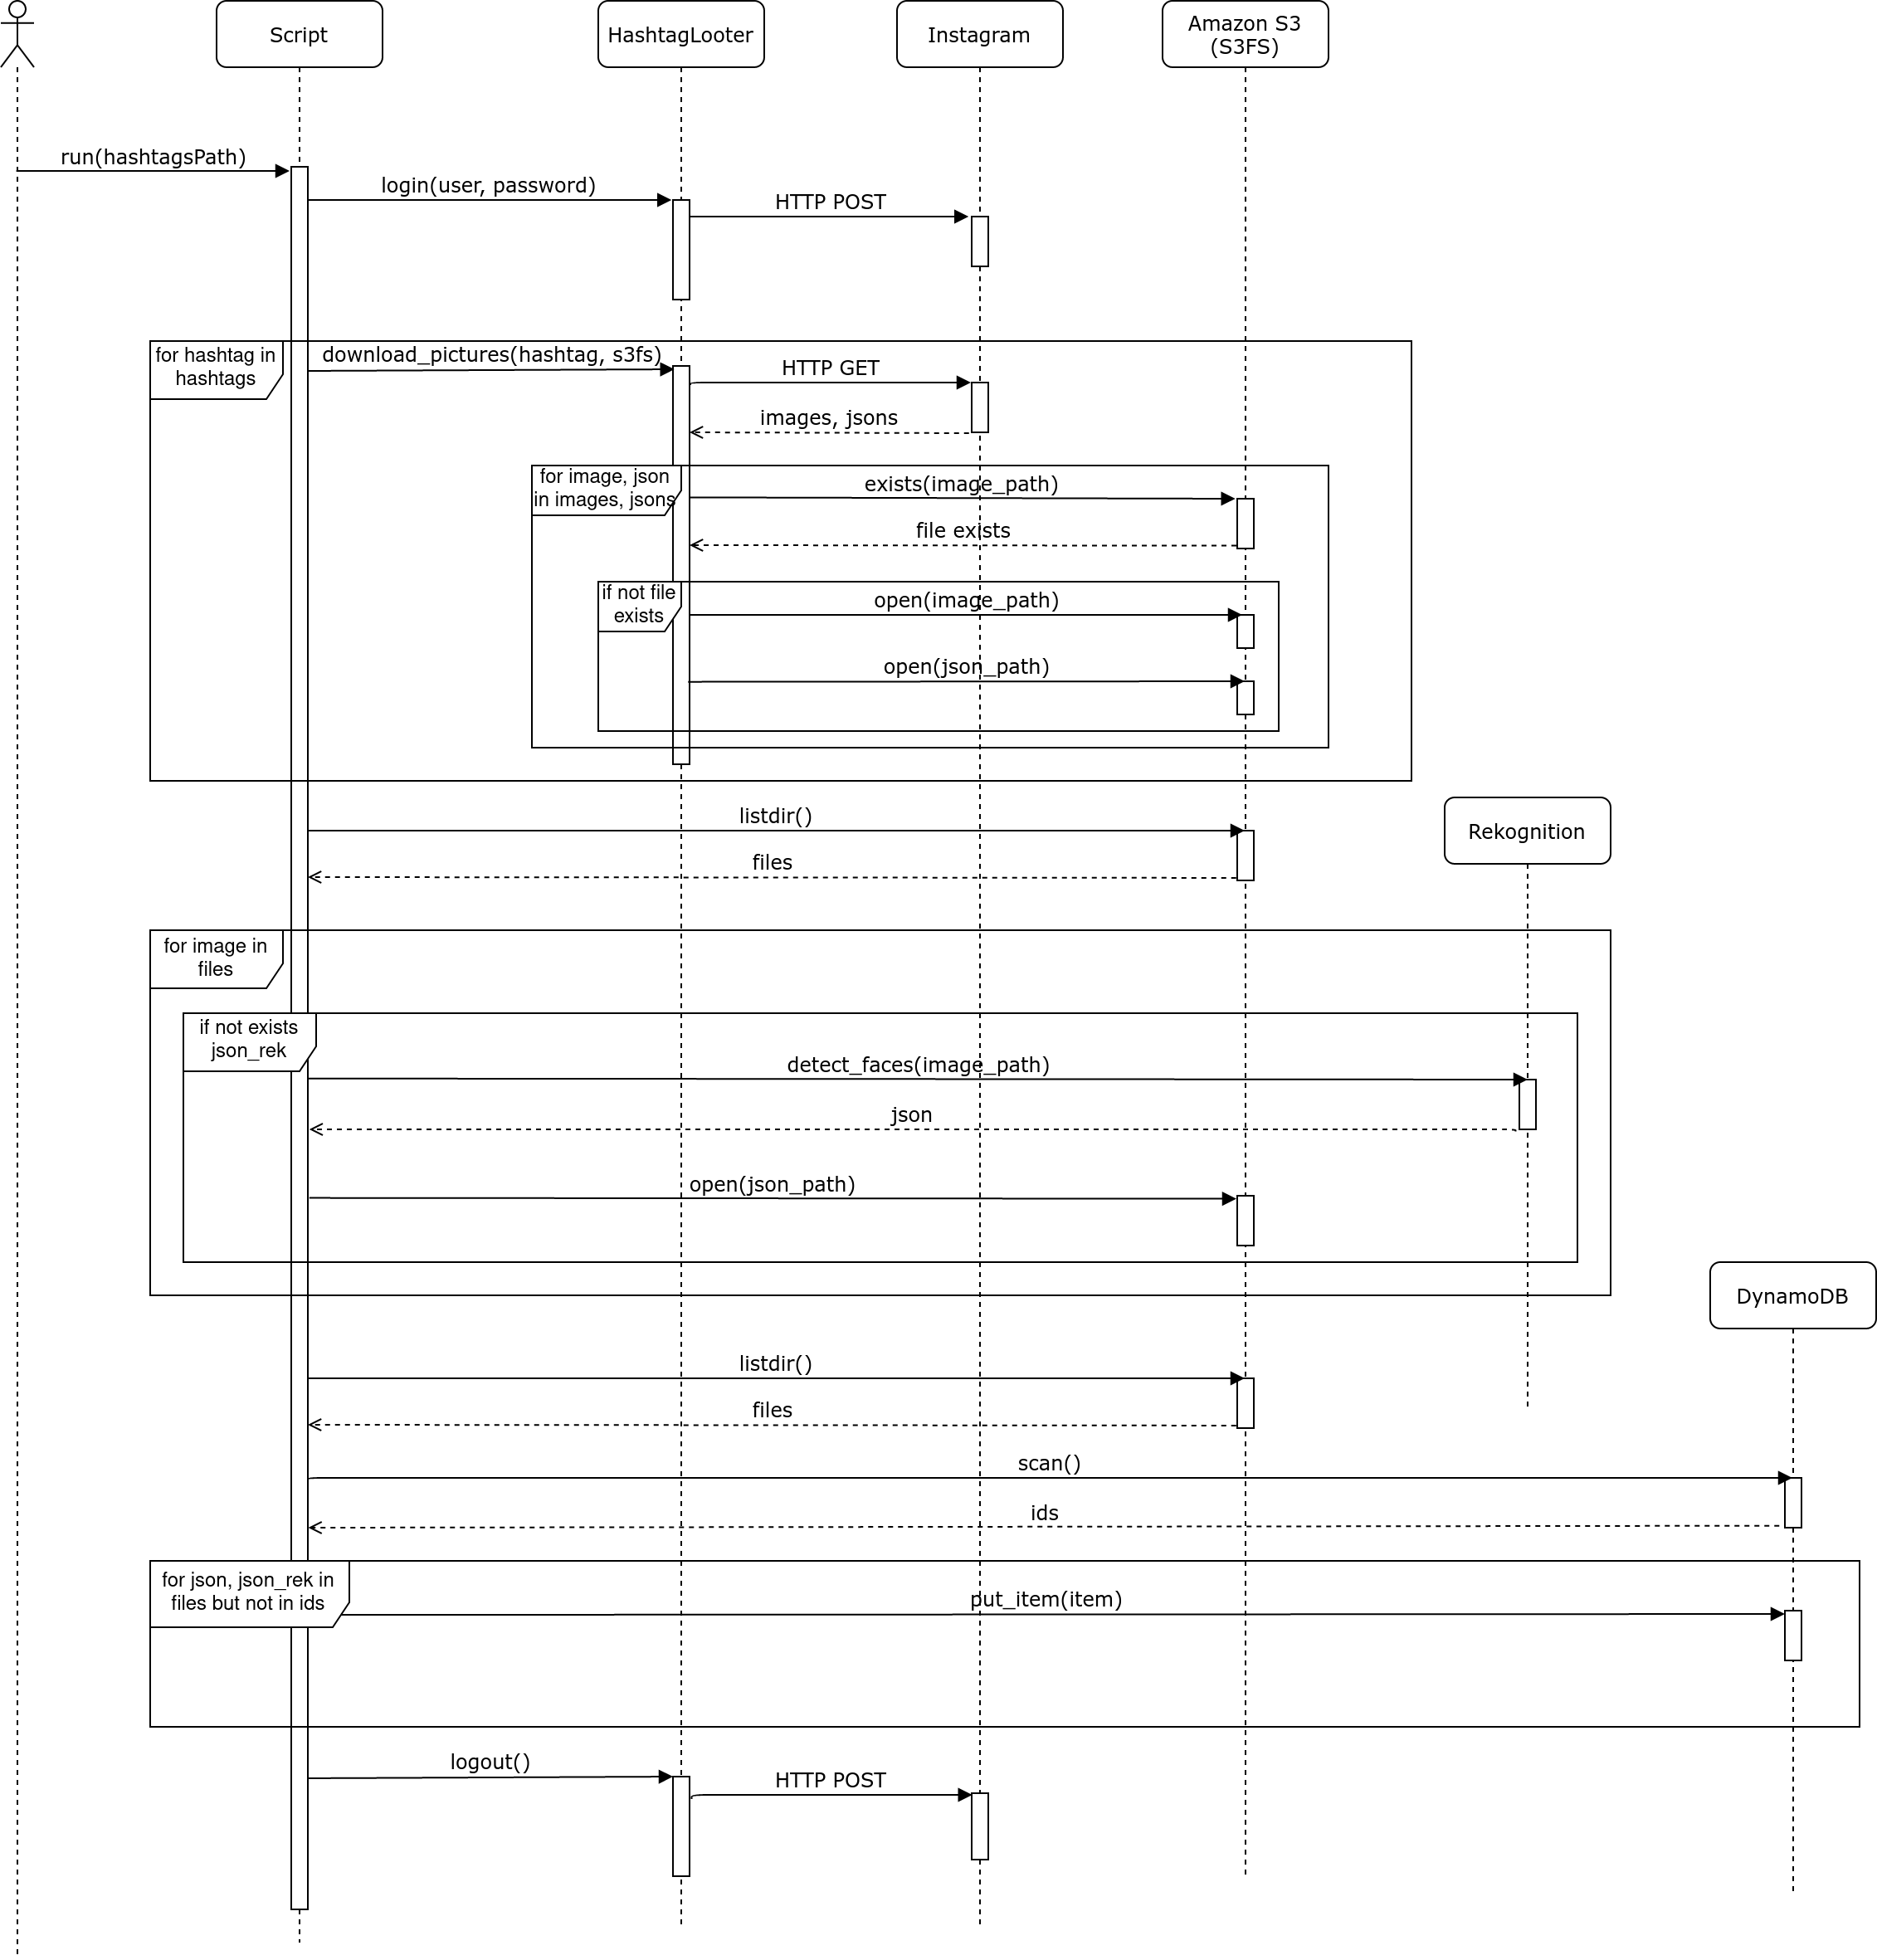
\includegraphics[width=1.25\textwidth]{sequence.drawio.png}
    \caption{Diagrama de secuencia de \texttt{mainScriptAWS.py}}
    \label{fig:sequence_script}
\end{figure}

Como se puede ver en el diagrama anterior, el script tan solo toma como argumento la ruta del fichero que contiene la lista de hashtags a consultar en Instagram (un hashtag por línea). El resto de identificadores y credenciales para acceder a Instagram o a los servicios de AWS han de estar definidos como variables de entorno.

\section{Proceso de descarga de las publicaciones}
\label{sect:descarga_publicaciones}

Para llevar a cabo el proceso de descarga de publicaciones y el poblado de la base de datos se tuvo que ejecutar el script de la sección anterior en varias ocasiones. El entorno de ejecución desde el que puso en funcionamiento siempre fue una máquina virtual, con Python 3, \texttt{virtualenv} y todas las librerías y SDKs instalados. Esta maquina virtual es una de las instancias que Amazon Web Services permite crear en su capa gratuita mediante su servicio EC2. Exactamente, la configuración escogida para esta instancia es la siguiente: 1 CPU \texttt{t2.micro}, 1 GB de RAM, 30 GBs de almacenamiento SSD, 100 GBs de ancho de banda con IP estática y el sistema operativo Debian 11 de 64 bits.

Sobre la lista de hashtags que se pasa al script como argumento, inicialmente se decidió obtener un número cercano a 50 hashtags relacionados con Valladolid y el turismo en Valladolid. Esta lista habría que obtenerla manualmente buscando en Instagram hashtags populares dentro de este contexto así como las etiquetas de las publicaciones encontradas. La lista finalmente creada consta de los siguientes 44 hashtags:

\begin{multicols}{3}
\begin{itemize}
	\item Naturaleza\_valladolid
	\item estaes\_valladolid
	\item valladolidturismooficial
	\item turismovalladolid
	\item valladolidturismo
	\item turismovalladolid
	\item valladolidspain
	\item valladolidfotos
	\item valladolidenfotos
	\item valladolid
	\item todo\_valladolid
	\item total\_valladolid
	\item igersvalladolid
	\item igervalladolid
	\item catedraldevalladolid
	\item paseandoporvalladolid
	\item valladolidgram
	\item instavalladolid
	\item valladolidlove
	\item valladolidlife
	\item valladolidmola
	\item megustavalladolid
	\item fotosdevalladolid
	\item valladolidhoy
	\item vallafotos
	\item valladolidinquieta
	\item love\_valladolid
	\item visitvalladolid
	\item look\_valladolid
	\item ok\_valladolid
	\item megustavalladolid
	\item asi\_es\_valladolid
	\item pucela
	\item megustapucela
	\item arquitecturavalladolid
	\item valladolidespaña
	\item culturavalladolid
	\item valladolidcapital
	\item valladolidcampogrande
	\item valladolidpaseozorrilla
	\item iglesiadelaantiguavalladolid
	\item igerspucela
	\item rinconesdevalladolid
	\item megustapucela
\end{itemize}
\end{multicols}

A la hora de ejecutar el script un detalle a tener en cuenta es el límite de publicaciones que podemos descargar y analizar en la capa gratuita. Al mes, en Rekognition se pueden analizar hasta 5000 imágenes, en DynamoDB se tiene un límite de 200 millones de solicitudes y en S3 existe un límite de 2000 solicitudes \textit{put}, siendo este último punto el mayor factor limitante. Debido a esto y al límite de la fecha de entrega del proyecto, en la base de datos finalmente generada se descargaron un total de 3916 publicaciones de Instagram. Tras el análisis con Rekognition, a partir de estas publicaciones se extrajeron unas 5408 caras.

Un detalle a destacar fue que, durante una de las ejecuciones del script, se detectó un problema a la hora de iniciar sesión en Instagram mediante Instalooter, impidiendo llevar a cabo el proceso de descarga de publicaciones. Tras revisar el error generado por el scraper y comprobar que este no era puntual, se llegó a la conclusión de que debió de haber alguna actualización en la web de Instagram que provocó que la librería dejara de funcionar correctamente. Revisando la pestaña de problemas en el repositorio de GitHub de la librería, se observó que es un error que le sucedía a más usuarios.

Como las últimas actualizaciones del repositorio de Instalooter fueron hace varios meses en el momento en que se hizo la comprobación, se decidió probar de nuevo otras librerías como \textit{Instaloader}, pero se llegó a la conclusión de que su uso era muy distinto a Instalooter y no ofrecía las ventajas de poder comprobar publicaciones ya descargadas y poder conectarlo de forma sencilla a los servicios en la nube. Es por ello que se decidió revisar el código fuente de la librería, y tras unas pruebas se consiguió dar con la fuente del error: un cambio en como se gestionaban las \textit{cookies} donde se guardan los \textit{tokens} empleados para logearse en la web. Como el cambio no era muy complicado se decidió corregirlo en un fork \url{https://github.com/Zalez95/InstaLooter.git} de la librería, y tras comprobar que funcionaba correctamente, se instaló mediante \texttt{pip3} en el entorno de la máquina virtual. Tras está corrección no volvió a dar problemas, y de hecho se hizo un \textit{pull request} a la librería original que en la actualidad está en proceso de revisión.

\section{Visualización}
\label{sect:grafana_visualizacion}

Una vez se han obtenido los datos necesarios para el proyecto, para poder usarlos de forma más cómoda se decidió que era necesario implementar algún tipo de visualización. Esta visualización debería permitir filtrar los datos de forma sencilla de acuerda a criterios como edad o género, y permitir seleccionar aquellas publicaciones que tuvieran un sentimiento positivo. También debería poder llevarnos fácilmente hasta las publicaciones mostradas en Instagram.

De acuerdo a las necesidades anteriores se llegó a la conclusión de que la forma más óptima de visualizar los datos era llevar a cabo algún tipo de cuadro de mandos. Para implementar un cuadro de mandos sobre una base de datos de DynamoDB se encontraron varias posibilidades:

\begin{enumerate}
    \item QLik: herramienta para crear dashboards con la que se ha trabajado anteriormente en este mismo máster, exactamente en la asignatura de Inteligencia de Negocio. No es una herramienta gratuita ni software libre, pero ofrece un periodo de prueba. El problema es que no se puede usar directamente con DynamoDB, sino que hay que usar un conector ODBC de la empresa Simba que no es gratuito.
    \item Microsoft PowerBI: Al igual que en la herramienta anterior, no es gratuito pero ofrece un periodo de prueba. Tampoco tiene conectores con DynamoDB, habría que usar el conector ODBC de Simba anteriormente comentado.
    \item Tableau: Ofrece un periodo de \textit{trial} de 3 meses, además existe una versión \textit{public} gratuita. Para usarlo junto con DynamoDB habría que usar el conector JDBC de Rockset que tampoco es gratuito (hay periodo de prueba pero no se indica durante cuanto tiempo).
    \item Grafana: Es open source pero no tiene conector gratuito con DynamoDB. Parece que tiene plugins que permiten conectarlo con servicios REST de forma sencilla. Se podría crear un conector creando un servidor que implementara estas APIs REST para acceder a DynamoDB como se hace en \cite{grafana_lambda_api}.
    \item Web estática junto con alguna librería para hacer gráficos: En esta opción habría que crear una página web estática manualmente y programar los gráficos en JavaScript mediante alguna librería como ChartJS o D3.js, conectándose con la base de datos a través del SDK de AWS para este lenguaje de programación. Un ejemplo de implementación se puede encontrar en \cite{web_chartjs}.
\end{enumerate}

Finalmente se decidió emplear Grafana aunque haya que implementar el conector, puesto que al ser open source no se tiene restricciones de tiempo de uso. Crear una página web estática desde cero o usando librerías consume mucho tiempo, y el resto de herramientas para hacer cuadros de mando también presentan el mismo problema a la hora de conectar con DynamoDB.

Para crear el cuadro de mandos con Grafana hubo que instalar Grafana Enterprise. En este caso se decidió hacerlo en la misma máquina virtual que se usa también para la ejecución del script de la sección anterior. Grafana es una aplicación web que por defecto se ejecuta en el puerto 3000, es por ello que para acceder desde fuera de este equipo hubo que abrir el puerto añadiendo una regla TCP en los grupos de seguridad de Amazon EC2. Una vez instalado Grafana y con el servicio corriendo, el siguiente paso fue instalar el plugin \texttt{JSON} para conectarse con fuentes de datos (\textit{data sources}) a través de HTTP. Para que este plugin funcione, el servidor al que se conecte ha de implementar una API REST con las siguientes operaciones:

\begin{itemize}
    \item \texttt{GET /} $\rightarrow$ Ha de devolver un código 200 OK si el servicio funciona correctamente.
    \item \texttt{POST /query} $\rightarrow$ Ha de devolver los valores pedidos. Para ello esta función tiene como parámetros un rango de fechas en el que se tienen que encontrar los datos, y da la posibilidad de filtrar por más valores mediante unos \textit{adhoc filters}. Los valores devueltos pueden estar en formato de tabla o en formato clave-valor, siendo la clave una fecha y el valor el contenido de una columna.
    \item \texttt{POST /search} $\rightarrow$ Ha de devolver las distintas métricas para llevar a cabo el filtrado, en nuestro caso se corresponde con el nombre de las columnas, o los posibles valores si como parámetro llega el nombre de una columna.
    \item \texttt{POST /tag-keys} $\rightarrow$ Ha de devolver las posibles claves para llevar a cabo el filtrado, en nuestro caso se corresponde con el nombre de las columnas.
    \item \texttt{POST /tag-values} $\rightarrow$ Ha de devolver los posibles valores de una clave para llevar a cabo el filtrado, en nuestro caso se corresponde con los valores distintos que hay para una columna.
\end{itemize}

Para poder crear el conector entre Grafana y DynamoDB hubo que hacer un servidor web que implementara las anteriores APIs, en este caso mediante Python 3 y el SDK de AWS \texttt{boto3}. Las pruebas iniciales se hicieron mediante un framework llamado \textit{bottle} para poder crear las APIs de forma local, y una vez que se comprobó que éstas funcionaban correctamente, se decidió implementar las APIs en Amazon Web Services para tener mejor rendimiento. Para implementar las APIs en AWS se usó sus servicios AWS Lambda, Amazon API Gateway y Amazon DynamoDB de la siguiente forma:

\begin{figure}[H]
    \centering
    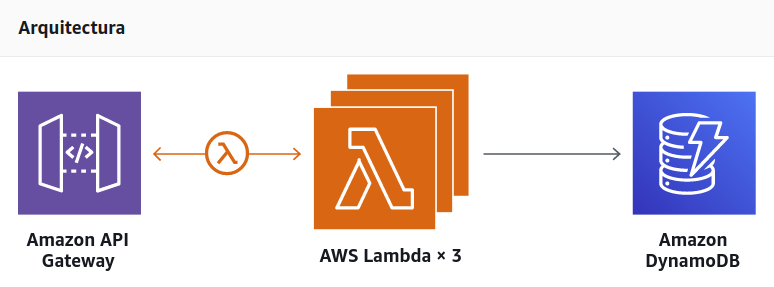
\includegraphics[width=0.9\textwidth]{gateway.png}
    \caption{Acceso a DynamoDB mediante APIs REST con API Gateway}
    \label{fig:gateway_schema}
\end{figure}

Siendo el diagrama de componentes del sistema completo el siguiente:

\begin{figure}[H]
    \hspace*{-1cm}
    \centering
    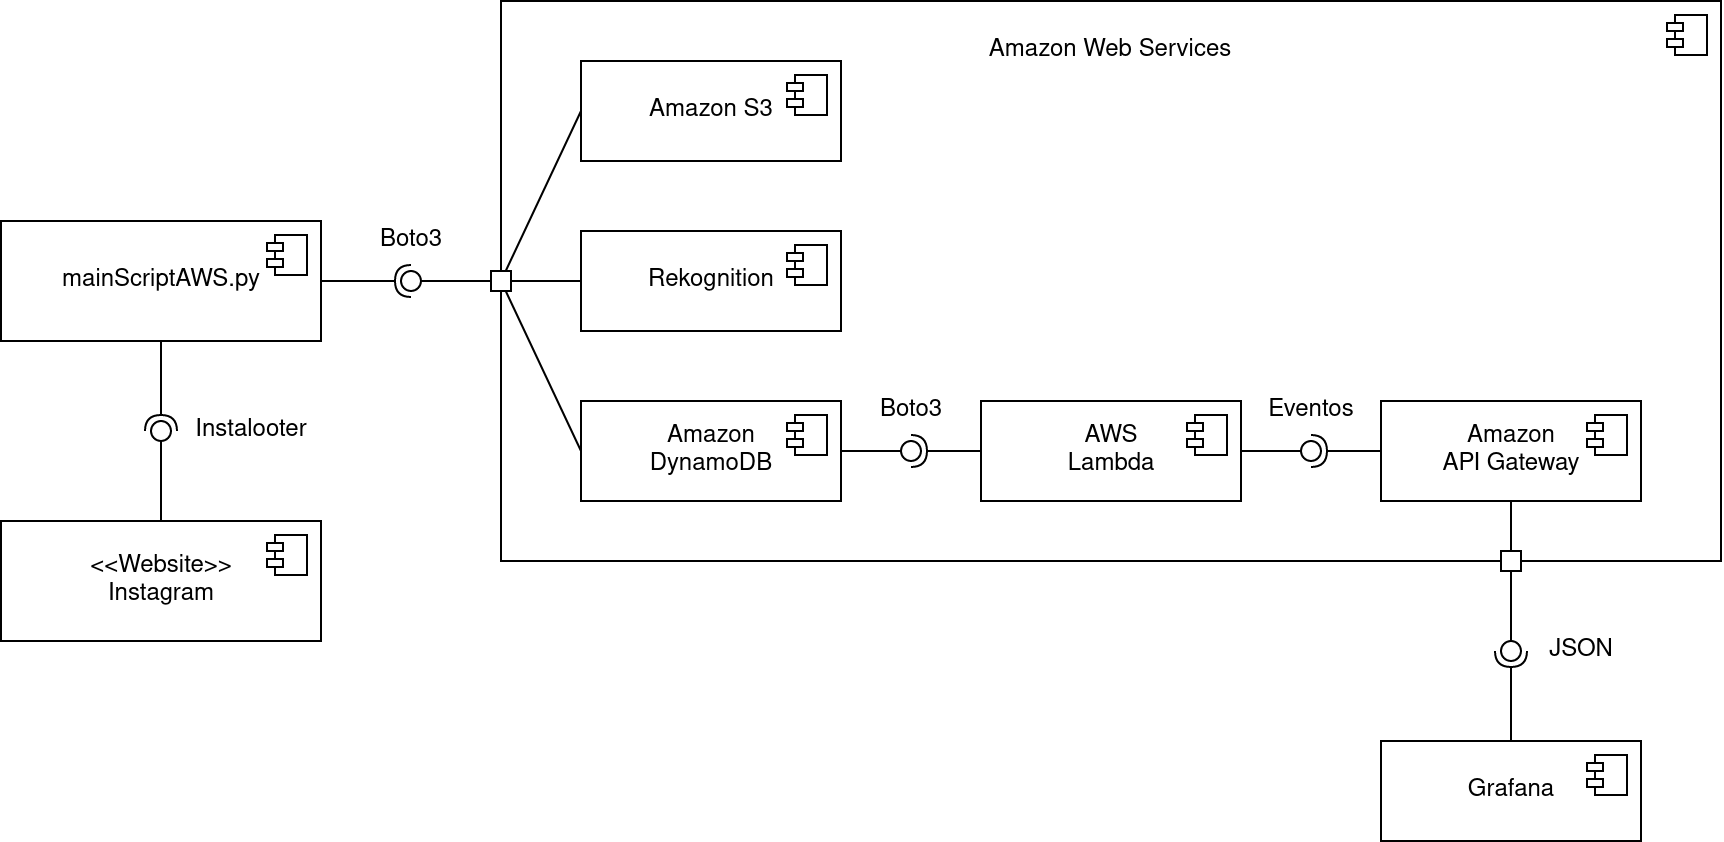
\includegraphics[width=1.2\textwidth]{memoria/img/component.drawio.png}
    \caption{Diagrama de Componentes del sistema}
    \label{fig:component_diag}
\end{figure}

AWS Lambda permite ejecutar código en la nube de Amazon sin tener que crear instancias de máquinas virtuales. En total se generaron 5 funciones para acceder a DynamoDB: \texttt{grafana\_query}, \texttt{grafana\_tagkeys}, \texttt{grafana\_helloworld}, \texttt{grafana\_tagvalues}, \texttt{grafana\_search}, implementando el acceso a DynamoDB y la lógica correspondiente. Todas estas funciones se ejecutan en un entorno Python 3.8 en equipos x86\_64, con un tiempo de ejecución de máximo 1 minuto. Por otro lado, API Gateway es el servicio que permite implementar de forma sencilla y escalable APIs RESTful o Websocket. En este caso las APIs REST se generaron como recursos que tienen asociado un método HTTP y un \textit{endpoint}, y que al ser accedidas ejecutan su correspondiente función de AWS Lambda:

\begin{figure}[H]
    \hspace*{-2cm}
    \centering
    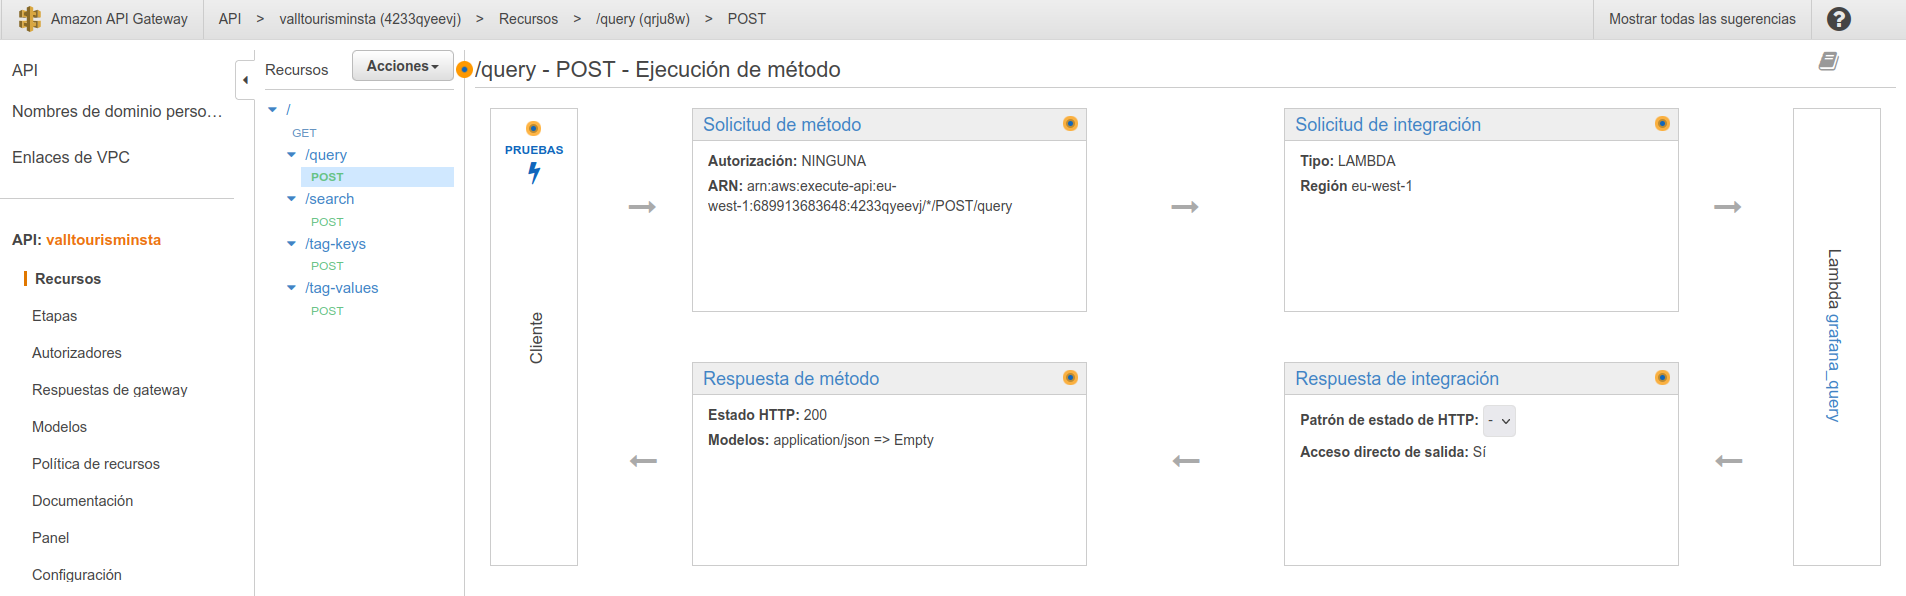
\includegraphics[width=1.25\textwidth]{gateway_cap.png}
    \caption{Configuración de AWS API Gateway y AWS Lambda}
    \label{fig:gateway_cap}
\end{figure}

Una vez que se crearon las APIs, el siguiente paso fue emplearlas con Grafana. Para ello se generó un \textit{data source} de tipo JSON que apuntaba a la URL del servicio de API Gateway. Tras conectar con éxito con la fuente de datos se procedió a la implementación del cuadro de mandos.

Para el diseño del dashboard se decidió emplear 3 columnas y 2 filas, ubicándose la información más relevante en la esquina superior izquierda puesto que está probado que las personas siguen un patrón en forma de Z a la hora visionar documentos o cuadros de mandos. El resultado final se puede ver en la figura \ref{fig:dashboard}.

En la esquina superior izquierda se muestra una combinación de estadísticas generales de las publicaciones mostradas, entre las que se encuentra el número de publicaciones mostradas, el número de caras y la proporción de genero de las caras mediante un gráfico de tarta. A su derecha se encuentra una tabla con información condensada de cada publicación, con un enlace hacia la publicación en Instagram, su fecha, la confianza, el género y la edad. Después, en la esquina superior derecha se muestra el número de publicaciones por fecha en un histograma para así poder ver que días hubo más publicaciones.

En la siguiente fila se muestra, a la izquierda la emoción predominante en todas las publicaciones, para ello se calcula el promedio de la confianza de cada emoción de todas las publicaciones y se muestra en un gráfico de tarta. A su derecha, el ``éxito'' de las publicaciones, en un histograma que muestra el promedio del número de comentarios y de likes que hubo cada día. Finalmente a su derecha se muestra la emoción promedio de las publicaciones por día.

\begin{figure}[H]
    \hspace*{-1.5cm}
    \centering
    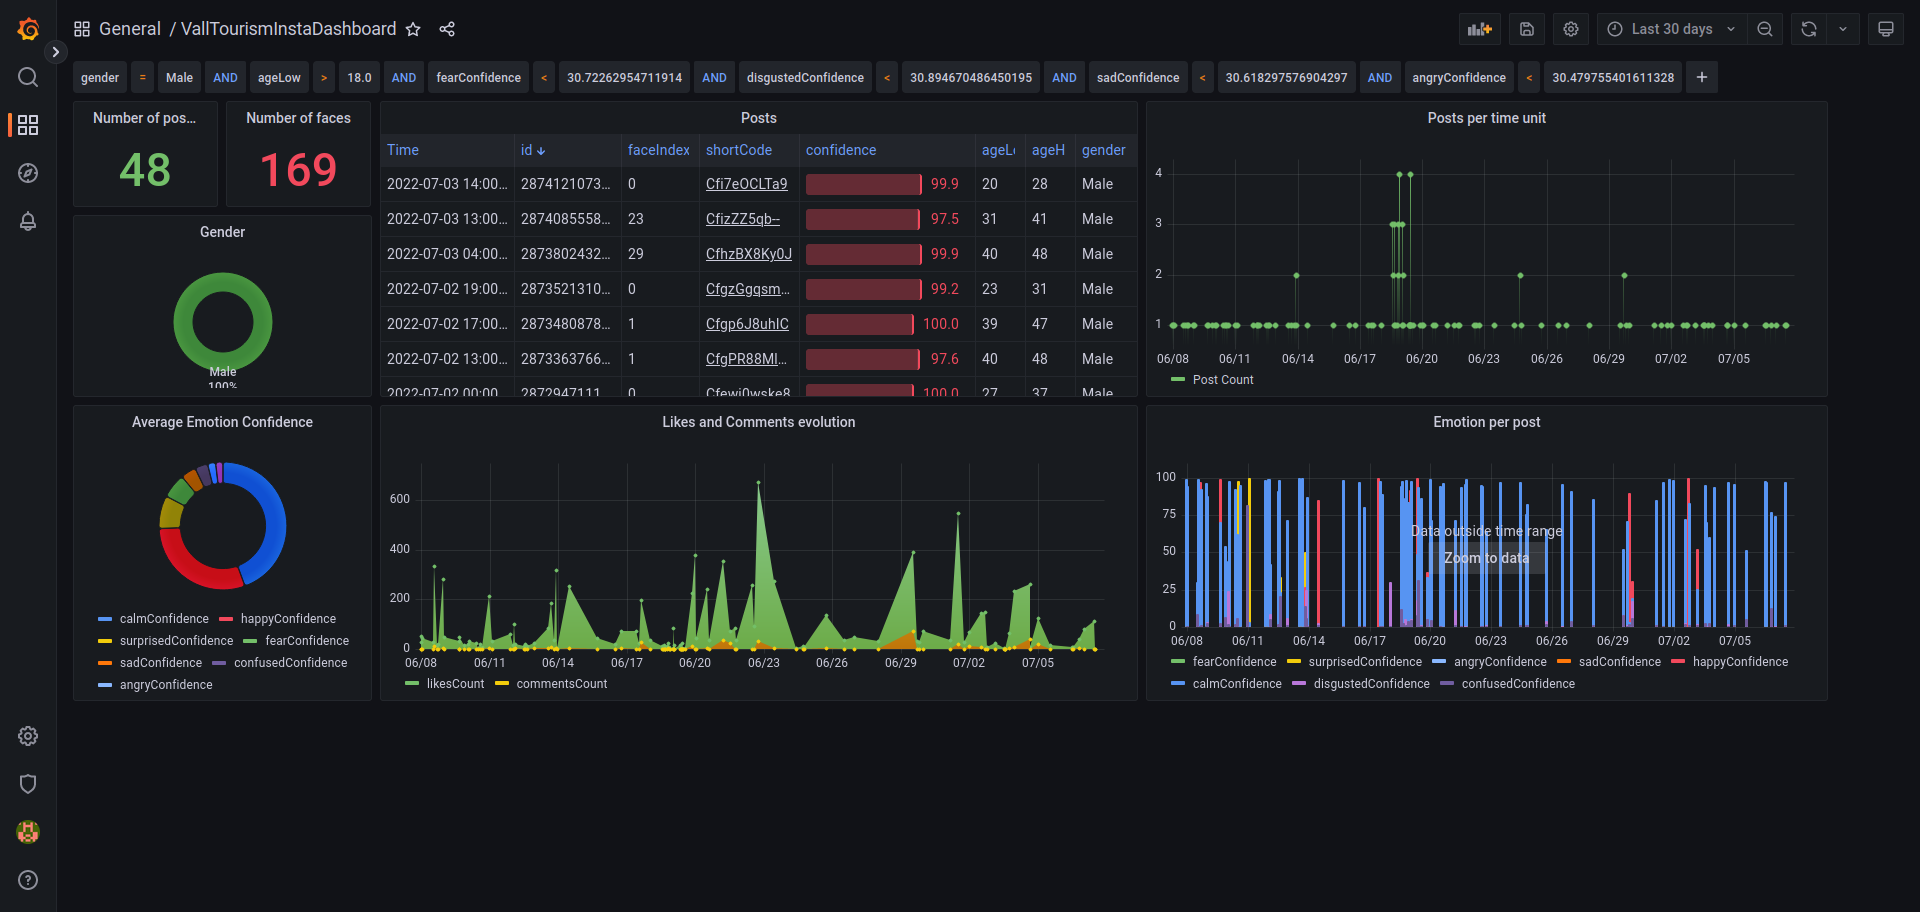
\includegraphics[width=1.3\textwidth]{dashboard.png}
    \caption{Cuadro de Mandos creado con Grafana}
    \label{fig:dashboard}
\end{figure}

Cabe destacar que Grafana muestra en la parte superior los distintos filtros a aplicar, por un lado las fechas, y por otro los filtros \textit{adhoc}, que pueden ser añadidos o modificados dinámicamente. En la captura anterior se puede ver que se están mostrando los últimos 30 días, y que se tienen habilitados varios filtros, exactamente género masculino, edad superior a los 18 años y se ha intentado que no haya emociones negativas predominantemente, descartando aquellas publicaciones que tengan una confianza superior al 30\% aproximadamente en las emociones triste, enfadado y disgustado.

\section{Acceso al proyecto}

Para concluir este apartado, se incluyen los enlaces a los distintos recursos desarrollados a lo largo del proyecto:

\begin{itemize}
    \item \href{https://github.com/Zalez95/TFM}{Enlace} de acceso público al repositorio del proyecto en GitHub.
    \item \href{http://3.250.43.138:3000/d/K0aCHsjnk/valltourisminstadashboard?orgId=1&from=1654898400000&to=1656885599000&var-filter1=gender%7C%3D%7CMale&var-filter1=ageLow%7C%3E%7C18.0&var-filter1=fearConfidence%7C%3C%7C30.72262954711914&var-filter1=disgustedConfidence%7C%3C%7C30.894670486450195&var-filter1=sadConfidence%7C%3C%7C30.618297576904297&var-filter1=angryConfidence%7C%3C%7C30.479755401611328}{Enlace} de acceso público al cuadro de mandos generado en la sección anterior, con los filtros indicados en la imagen \ref{fig:dashboard}.
\end{itemize}

